\documentclass[10pt,a4paper,twoside]{article}
\usepackage[dutch]{babel}
\usepackage[utf8]{inputenc}
\usepackage{amsmath}
\usepackage{graphicx}
\graphicspath{ {./dbms/} }
\usepackage{float,flafter}
\usepackage{hyperref}
\usepackage{inputenc}

\setlength\paperwidth{20.999cm}\setlength\paperheight{29.699cm}\setlength\voffset{-1in}\setlength\hoffset{-1in}\setlength\topmargin{1.499cm}\setlength\headheight{12pt}\setlength\headsep{0cm}\setlength\footskip{1.131cm}\setlength\textheight{25cm}\setlength\oddsidemargin{2.499cm}\setlength\textwidth{15.999cm}

\begin{document}

\begin{center}
\hrule

\vspace{.4cm}
{\bf {\Large TERM PAPER  }}\\
\vspace{.3cm}
{\bf {\huge Big data management challenges in healthcare }}
\vspace{.3cm}
\end{center}

{\bf Name:}  Priyanshu Gupta

{\bf Roll no:}  19111042 

{\bf Branch: } 6th Biomedical Engineering, 2022 
\\
\hrule

\vspace{.3cm}
\section*{Introduction} 
What is Big data?\\
Big Data is a term used for addressing a huge and heterogeneous amount of data too large to be handled with common software systems. The information contained by this data set can be classified into various groups and many dimensions. Such versatile databases are fragile enough and immense in volume requiring a powerful and dynamic management system including software, infrastructure to meet today’s demand and privacy plus security concerns. Besides these, management should be powerful enough to make it available in real time, which will allow it to be analysed and used immediately. \\
 
\textbf{Big data in healthcare}\\
A similar demand follows in the healthcare systems. At every level of medical care, the different kind of information either be it a patient’s medical history or a medical and clinical data, everything is equally informative for next surgery or appointment. Also it is a tedious job to maintain each and every hardcopy of a person’s medical history and present when ever needed. Due to this need, a new system Electronic health records (EHR) was introduced which represent records maintained electronically for improving the health care sector towards the benefit of patients and clinicians. In the era of telemedicine with so much advancement in computer systems, the digitalization of medicine along with medical records and all clinical test and experiment reports is becoming a standard. Nowadays, every single information is working through cloud and healthcare is becoming one such discipline. This information from clinical studies, research and observations of individuals’ lifestyle and environmental exposure are all of great value towards advanced health research, since they work as a training datasets for predictive models for the solution and ease of real life biomedical problems. The increasing availability of omics data from a single blood test to surgeries and research reports contributing to the Big data is becoming a major challenge across health research disciplines.    \\


\begin{center}
    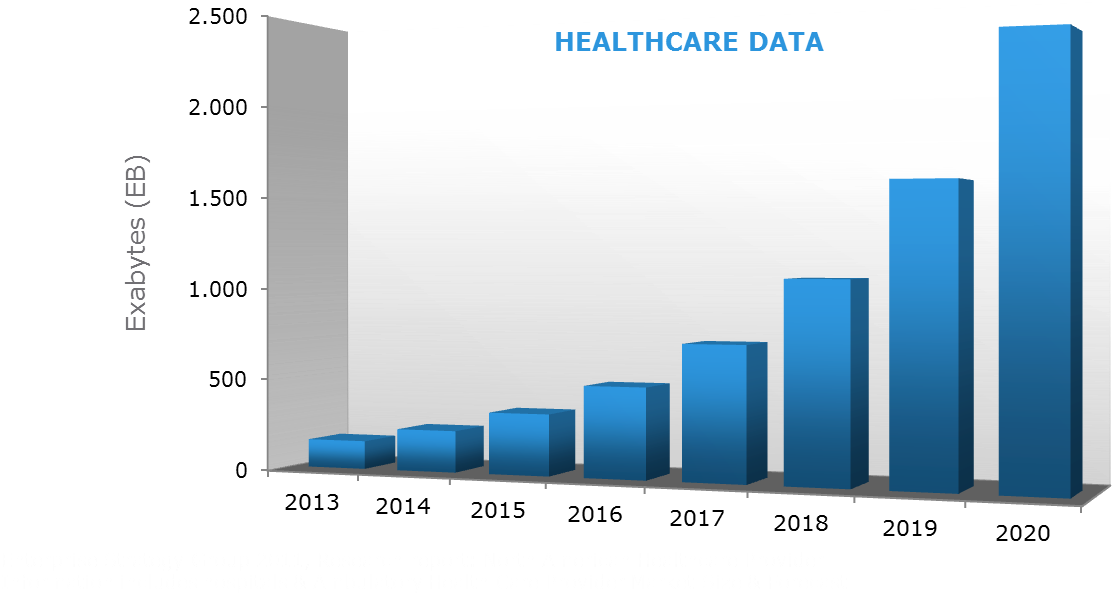
\includegraphics[width=15cm, height=8cm]{healthcaredata} \\[\baselineskip]
\end{center}

\section*{Challenges associated with healthcare big data }
\textbf{Current data management practice in health research }

The huge and heterogeneous big data in healthcare is less informative with normal database systems. The common software frameworks for operating big data analysis are high power computing clusters that are accessible via grid computing infrastructures. \textbf{Apache Hadoop} is an open source software framework for large-scale storing and processing of big data. Hadoop comprises of two components, Hadoop Distributed File system (HDFS) and MapReduce. The latter one is used to partition the input into smaller sub problems by a master process and then distribute it to worker processes. It was used in the bioinformatics field under the project on “The Cancer Genome Atlas”. The process of “sharding” i.e. splitting genome data into smaller more manageable chunks was carried out using the Hadoop framework together with the Genome Analysis Toolkit. Another framework based on Hadoop is the \textbf{Apache Hive}. It is a distributed data warehouse infrastructure that supports data summarization, query and analysis of large datasets stored in (HDFS).

\begin{center}
    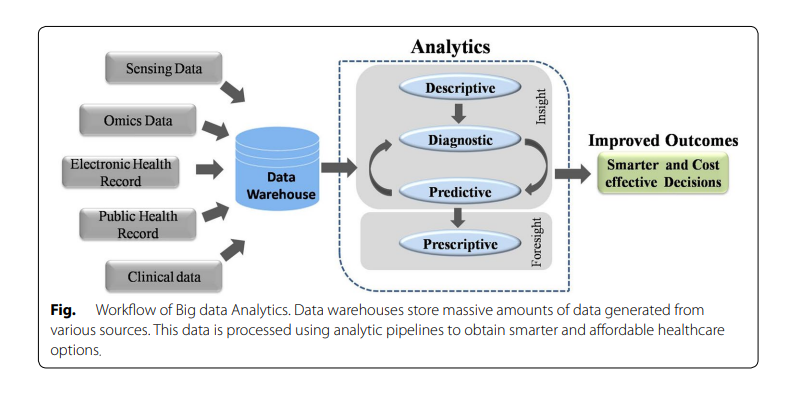
\includegraphics[width=16cm, height=9cm]{analytics} \\[\baselineskip]
\end{center}

For healthcare, the data gathered from various sources is mostly required for optimizing consumer services rather than consumer consumption. The heterogeneity, the noise and variety of the experimental techniques and the biological conditions these data should be considered, before integration in the database. Later on, different data mining techniques could be applied on these datasets such as: anomaly detection, clustering, classification, association rules summarization and visualization of these big data sets. These tools can help extract knowledge from patients’ care data to analysis and suggest innovative services to save their lives and to develop innovative techniques to diagnose and treat various diseases.
\\[\baselineskip]

\textbf{Data management approaches }\\
In biomedical data capture and archiving practice, both RDBMS and NoSQL DBMS have been used to build database tools. 
\begin{itemize}
 \item \textbf{The relational database RDBMS:} This is often used for information integration or normalisation. The SQL approach can develop data structures with Atomicity, Consistency, Isolation and Durability (ACID). The database flexibility and scalability of the SQL approach rely on a clean separation between data structure and data values, as well as correct identification and construction of data relations and relationships. The final product of this process is an executable database schema, in which all the atomic data elements (i.e. attributes) are meant to be highly reusable so that the schema can be relatively stable and generalizable across studies. The relational database models (RDBMS) are not suitable for Big Data problems because they lack horizontal scalability and need hard consistency and become very complex when representing structured relationships.

 \item \textbf{The non-relational approaches: }This is for information centralisation. The NoSQL solutions focus on data availability, so they generally do not require rigorous data attribute atomicity (i.e. normalization) nor demand predefined data relationship. Therefore, these are often referred to as ‘open schema’ or ‘schema-flexible’. Even if the NoSQL approach has proven to be a potent solution for information centralization and target finding, especially in big data applications, the inability to query granular-level semi-structured or unstructured data is a common problem with NoSQL repositories in the biomedical data space. In that situation, users have to download the entire data set to figure out details on their own.
 
\end{itemize}

\end{document}
